\documentclass{subfiles}
\begin{document}
    \begin{figure}[!hb]
        \centering
        \begin{subfigure}{0.45\textwidth}
            \centering
            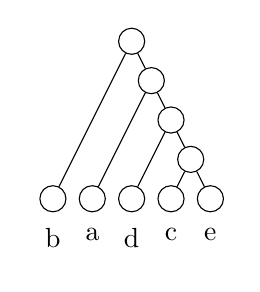
\begin{tikzpicture}[
                every node/.style={draw, circle, minimum size=0.1cm},
                scale = 0.5    
            ]

                \node (root) at (0, 0) {};
                \foreach \sym/\pos in {a/-1, b/-2, c/1, d/0, e/2} {
                    \node (\sym) at (\pos, -4) [label=below:\sym] {};
                }

                \node (m1) at (1.5, -3) {};
                \node (m2) at (1, -2) {};
                \node (m3) at (0.5, -1) {};

                \draw (e) -- (m1) -- (c);
                \draw (d) -- (m2) -- (m1);
                \draw (a) -- (m3) -- (m2);
                \draw (b) -- (root) -- (m3);
            \end{tikzpicture}
        \end{subfigure}
        \begin{subfigure}{0.45\textwidth}
            \centering
            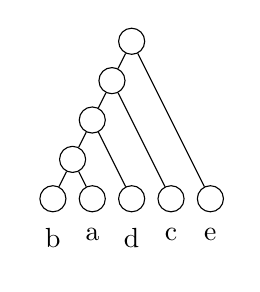
\begin{tikzpicture}[
                every node/.style={draw, circle, minimum size=0.1cm},
                scale = 0.5    
            ]

                \node (root) at (0, 0) {};
                \foreach \sym/\pos in {a/-1, b/-2, c/1, d/0, e/2} {
                    \node (\sym) at (\pos, -4) [label=below:\sym] {};
                }

                \node (m1) at (-1.5, -3) {};
                \node (m2) at (-1, -2) {};
                \node (m3) at (-0.5, -1) {};

                \draw (b) -- (m1) -- (a);
                \draw (d) -- (m2) -- (m1);
                \draw (c) -- (m3) -- (m2);
                \draw (e) -- (root) -- (m3);
            \end{tikzpicture}
        \end{subfigure}
    \end{figure}
\end{document}
